% Created 2019-11-03 dom 22:14
\documentclass[11pt]{article}
\usepackage[utf8]{inputenc}
\usepackage[T1]{fontenc}
\usepackage{fixltx2e}
\usepackage{graphicx}
\usepackage{longtable}
\usepackage{float}
\usepackage{wrapfig}
\usepackage{rotating}
\usepackage[normalem]{ulem}
\usepackage{amsmath}
\usepackage{textcomp}
\usepackage{marvosym}
\usepackage{wasysym}
\usepackage{amssymb}
\usepackage{hyperref}
\tolerance=1000
\hypersetup{colorlinks=true,linkcolor=black}
\author{Angel Berlanas}
\date{\today}
\title{UD02 - Transiciones CSS}
\hypersetup{
  pdfkeywords={},
  pdfsubject={},
  pdfcreator={Emacs 25.2.2 (Org mode 8.2.10)}}
\begin{document}

\maketitle
\tableofcontents


\section{Transiciones CSS}
\label{sec-1}

\subsection{¿Qué son las transiciones CSS?}
\label{sec-1-1}

La manera más sencilla de animar elementos del DOM es utilizando Transiciones CSS. 
En esta unidad veremos como funcionan estas transiciones CSS y como utilizarlas en 
nuestras páginas web.

\subsection{Propiedades}
\label{sec-1-2}

A continuación vamos a ver las diferentes propiedades que puede tener una transición 
CSS, tener en cuenta que muchos de los conceptos que se vean aquí se \textbf{re-aprovecharán} en 
las \textbf{Animaciones CSS}.

\subsubsection{transition-property}
\label{sec-1-2-1}


Se trata de la propiedad que vamos a transicionar, o que va a cambiar en la
transición, ya sea el \verb~background-color~ o \verb~width~. 

\begin{verbatim}
.transicionable{
     transition-property: background-color;
}

.transicionado{
     background-color: #FABADA;
}
\end{verbatim}

Cuando a un elemento del DOM que tenga la clase \verb~transicionable~ se le aplique
la clase \verb~transicionado~ el color de fondo del elemento cambiará.

Los siguientes atributos se encargan de modificar \emph{cómo} se realizará ese cambio
de las propiedades que \emph{transicionan}.

\subsubsection{transition-duration}
\label{sec-1-2-2}

Esta propiedad indica el número de segundos (\verb~s~) que dura la transición. Se
trata de un parámetro \textbf{requerido} si usamos la propiedad combinada (ver más
adelante).

\begin{verbatim}
.transicionable{
     transition-property: background-color;
     transition-duration: 2s;
}

.transicionado{
     background-color: #FABADA;
}
\end{verbatim}

\subsubsection{transition-timing-function}
\label{sec-1-2-3}


Uno de los conceptos más complicados y que merecen más explicación, no es
sencillo de explicar, pero intentaremos acercarnos lo más posible.

\begin{verbatim}
.transicionable{

     background-color: blue;

     transition-property: background-color;
     transition-duration: 2s;
     transition-timing-function: linear; 
}

.transicionable:hover{
     background-color: #FABADA;
}
\end{verbatim}

En este caso, lo que ocurre es que cambia el color de manera \emph{constante} a lo
largo de los dos segundos que dura la transición. Si lo reproducís en vuestro
navegador, previo paso de crear los ficheros necesarios, vereis como al poner
encima el cursor del elemento, va cambiando de color de manera constante hasta
llegar al color \verb~#FABADA~.

Esto en los cambios de color no se aprecia tanto, pero vamos a ver ahora una
transición un pelín diferente, un cambio de posición respecto a la posición en
\textbf{X}. 

La modificación de la \emph{velocidad} de transición nos permite dar efectos con más
presencia en la naturaleza, lo que hace que la experiencia del usuario sea más
confortable al ser más \emph{cercana a la realidad}. Un ejemplo de esto es que si
tenemos que desplazar un elemento desde una posición a otra en una ventana, el
usuario verá más \emph{natural} que el movimiento comience lento, acelere y luego
frene al llegar a su destino, de la misma manera que lo hacemos nosotros y
podemos observarlo en el mundo real.

Para much@s esta diferencia es muy sutil, pero puede ser la diferencia entre un
diseño muy bueno y otro excelente.

\begin{figure}[htb]
\centering
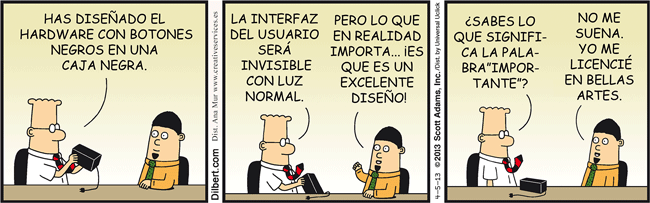
\includegraphics[width=.9\linewidth]{./imgs/dilbert_disenyo.png}
\caption{\label{fig:-Dilbert_001}El diseño según Dilbert}
\end{figure}


Para abordar con éxito el ejemplo presentaremos dos conceptos que ayudarán a
comprenderlo mejor.

\begin{itemize}
\item transition: transform;
\item transform: translateX(Npx);
\end{itemize}

\subsubsection{transform}
\label{sec-1-2-4}

Es una propiedad \verb~css~ que nos permite modificar el espacio de coordenadas
del modelo de formato visual CSS. Usándola, los elementos pueden ser
trasladados, rotados, escalados o sesgados de acuerdo a los valores
establecidos

Se trata de una de las propiedades más usadas en las las transiciones y
animaciones, ya que nos permite mover los elementos a diferentes puntos de
la ventana desde el CSS.

\verb~transform~ presenta muchas posibilidades, pero para este ejemplo nos
centraremos en una muy sencilla: \verb~translateX~.

\subsubsection{translateX}
\label{sec-1-2-5}

Esta transformación \emph{reposiciona} un elemento horizontalmente en un plano
2D. Veremos algunos ejemplos de esto más adelante.

\begin{verbatim}
/* <length-percentage> values */
transform: translateX(200px);
transform: translateX(50%);
\end{verbatim}

Esto desplazará el objeto \verb~200px~ hacia la derecha y en el caso de la segunda
opción lo trasladará la mitad de la pantalla.

Una vez explicadas estas dos propiedades, continuamos con la explicación de
las diferentes formas de \emph{animar} una transición. Volvamos a
\textbf{transition-timing-function}.

\subsubsection{Diferentes valores para transition-timing-function}
\label{sec-1-2-6}

\begin{enumerate}
\item ease-out
\label{sec-1-2-6-1}

Representa el efecto de ir deteniéndose paulatinamente antes de llegar al
destino, como si se acabara el impulso.

\item ease-in
\label{sec-1-2-6-2}

En este caso la animación \emph{acelerará} hasta llegar a una velocidad de
crucero y acabará la animación a esa velocidad.

\item ease-in-out
\label{sec-1-2-6-3}

Una combinación de ambas, representa el inicio lento, acelerar, y luego
frenar cuando esté cerca del final.

\item cubic-bezier
\label{sec-1-2-6-4}

Si las combinaciones anteriores no acaban de ajustarse al efecto que
necesitamos, o sencillamente se nos pide que sea de otra manera, por
ejemplo : \emph{rápido-lento-rápido}, deberemos \verb~programar~ nuestra propia
animación haciendo uso de las \verb~curvas-bezier~.

Esto lo veremos más adelante en esta unidad, pero ahora vamos a realizar
unos ejercicios para afianzar lo aprendido.
\end{enumerate}

\subsubsection{Ejercicio 10}
\label{sec-1-2-7}

Utilizando el código fuente suministrado, crear o realizar los 
cambios corriespondientes en los ficheros :

\begin{itemize}
\item base.css
\item script.js
\end{itemize}

Para que los diferentes Cthulhus transicionen con los diferentes valores
vistos hasta ahora al pulsar el botón.

\begin{figure}[!h]
\centering
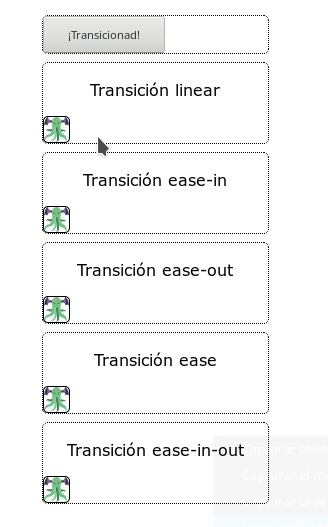
\includegraphics[width=100px]{./imgs/Tarea_10_1.png}
\caption{\label{fig:Tarea10_1}Ejercicio 10 : Inicio}
\end{figure}

\begin{figure}[!h]
\centering
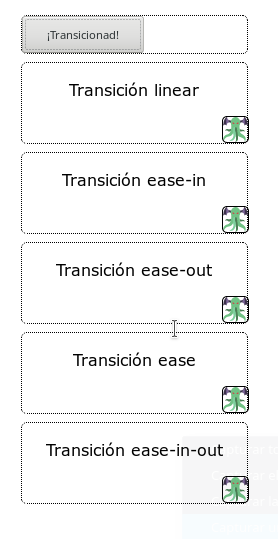
\includegraphics[width=100px]{./imgs/Tarea_10_2.png}
\caption{\label{fig:Tarea10_2}Ejercicio 10 : Fin}
\end{figure}

\begin{enumerate}
\item SubMisión 01:
\label{sec-1-2-7-1}

El código asociado a las clases \verb~css~: ease, ease-in, ease-out,
ease-in-out, tan solo se compone de 1 línea.

\item SubMisión 02:
\label{sec-1-2-7-2}

El código JS es tan solo una línea de código, sin \verb~;~. Para ello, se puede
utilizar las funciones lambda.
\end{enumerate}


\subsubsection{cubic-bezier}
\label{sec-1-2-8}

Las curvas bezier, es una notación que se utilizan en multitud de programas
de diseño 3D y 2D como el AutoCAD o Gimp que indican como se deben modificar
unas curvas para adaptarse a una determinada función.

No es \emph{relevante} que seamos capaces de crear nosotros los números que
forman la función \emph{bezier} de manera manual, para ello contamos las
\emph{herramientas de developers} en los navegadores que nos permiten crear
nuestras \emph{curvas bezier} de forma gráfica.

\url{https://developer.mozilla.org/es/docs/Web/CSS/Herramientas/Cubic_Bezier_Generator}


Esto nos permite crear animaciones mucho más personalizadas.

\subsubsection{Ejercicio 11}
\label{sec-1-2-9}

Utilizando el código fuente del ejercicio anterior, sustituye las palabras
clave de la transición: \verb~ease,ease-in,ease-out,ease-in-out y linear~ por una
llamada a la función \verb~cubic-bezier~ manteniendo la misma \textbf{UX (\emph{User
Expierence} )}.

\subsubsection{Transicionando 2 o más propriedades}
\label{sec-1-2-10}

Podemos \emph{transicionar} 2 (o más) propiedades \verb~CSS~ separandolas mediante una
coma (\textasciitilde{},\textasciitilde{}), en la propiedad \verb~transition~ o \verb~transition-property~.

\begin{verbatim}
.selector {
  transition: background-color 1s ease-out,
	      color 1s ease-out;

  /* O tambien */
  transition-property: background, color;
  transition-duration: 1s;
  transition-timing-function: ease-out;
}
\end{verbatim}

Podemos vernos tentandos de hacer lo siguiente:

\begin{verbatim}
/* NUNCA HAGAIS ESTO */
.selector {
  transition-property: all
}

/* ESTO ESTA BIEN */
.selector {
  transition-property: background-color, color, transform;
}
\end{verbatim}

Esto es debido a que tendrá un impacto \emph{muy negativo} en el rendimiento de
las transiciones, al igual que pasa con las excepciones de \verb~try-catch~ en
Java, cuanto más cerca estés del \emph{problema}, más fácilmente el motor genera
el código adecuado y es capaz de trabajar con la transición (\emph{o la
excepción,\ldots{}}).

\begin{figure}[!h]
\centering
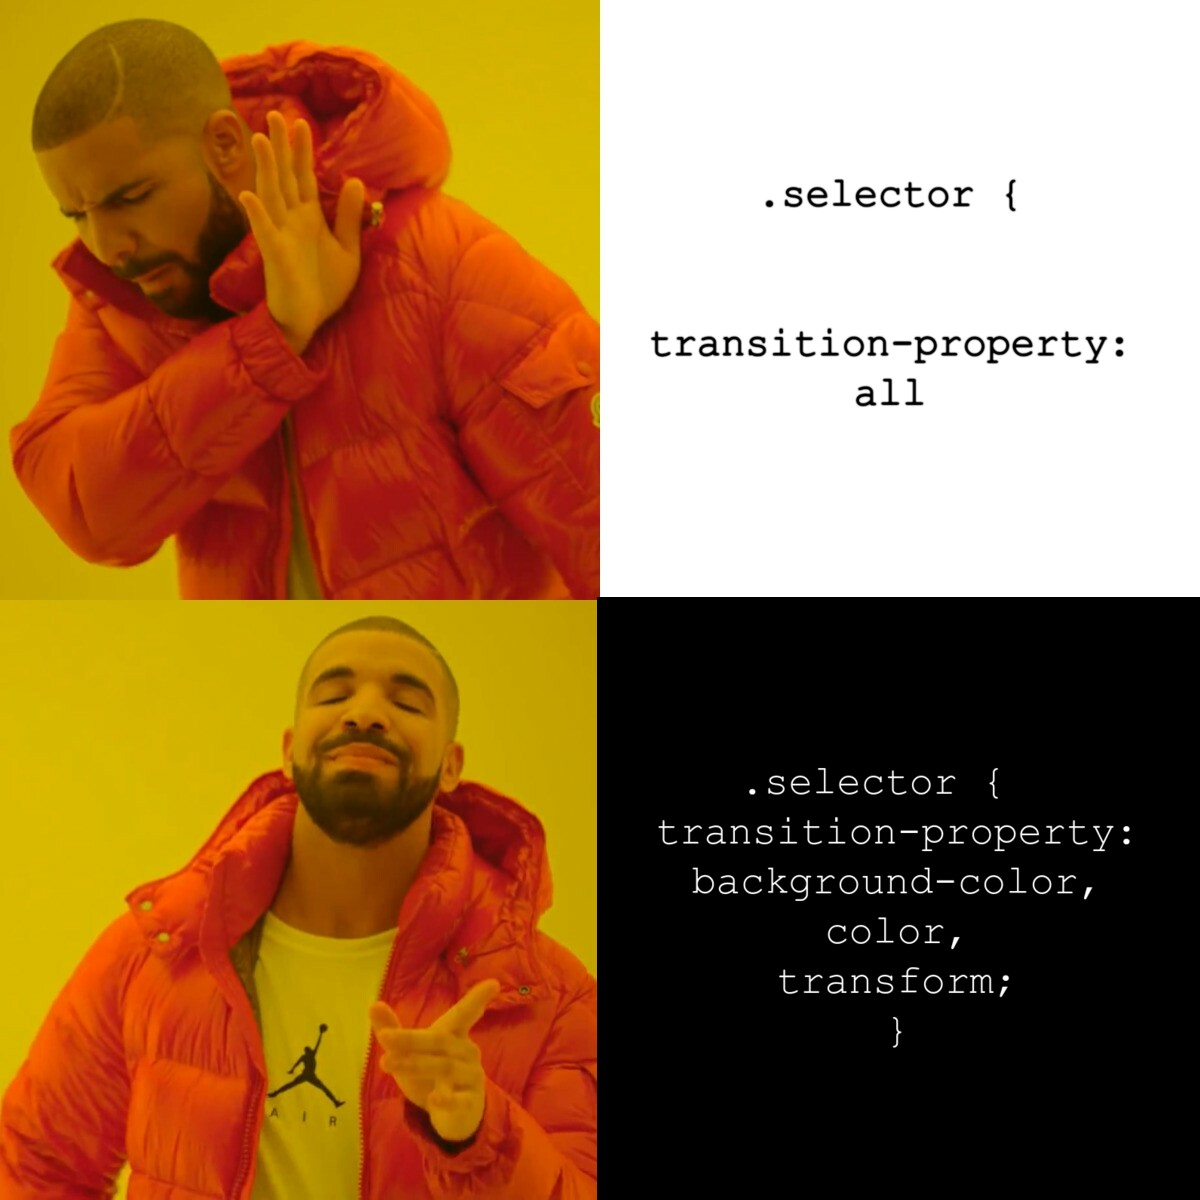
\includegraphics[width=.9\linewidth]{./imgs/transitionPropertyMeme.jpg}
\caption{\label{fig:transitionPropertyMeme}Como hacer las transiciones}
\end{figure}


\subsubsection{transition-delay}
\label{sec-1-2-11}

Por último la propiedad \verb~transition-delay~ nos permite especificar un tiempo
de espera para realizar la transición \emph{después} de que el cambio haya sido
realizado en el código.


\begin{verbatim}
.transicionable{
     transition-delay: 1s;
}
\end{verbatim}


\newpage
\subsubsection{Ejercicio 12 : Restaurando pergaminos}
\label{sec-1-2-12}

En el antiguo Egipto se le rendia culto a \emph{Sedefkar} un sacerdote que según
cuenta la leyenda, era capaz de invocar a peligrosas  criaturas que
realizaban pequeñas tareas para mantener el inmenso poder de \emph{Sedefkar}.

\begin{figure}[!h]
\centering

\includegraphics[width=200px]{./imgs/pergamino.jpg}
\caption{\label{fig:restaurandoElPergamino}Ejercicio 12 - Restaurando el pergamino}
\end{figure}

En las últimas semanas se ha encontrado un pergamino que contiene una
plantilla que puede usarse para volver a invocar a los \emph{Seres de Sedefkar}.

Sin embargo el tiempo ha hecho mella en el pergamino y se han perdido
fragmentos de los otros dos pergaminos a los que hace referencia ese pergamino, uno escrito en
la lengua de los antiguos Dioses (\verb~JS~) y otro pertenciente a la \emph{Casta}
\emph{Sacerdotal de Sedefkar} (\verb~CSS~).

\begin{enumerate}
\item Tareas:
\label{sec-1-2-12-1}

Se pide a los investigadores que recompongan los pergaminos, sabiendo lo
debe pasar con los seres invocados.

\begin{itemize}
\item Cuando se pulse el botón, debe aparecer una \verb~caja~. Esta se encuentra en un
estado latente, esperando.
\item Si se pulsa sobre la \verb~caja~, esta \emph{despierta}, moviendose hacia la
izquierda hasta situarse sobre otra caja (si la hubiera) y cambia su color.
\item Si se vuelve a pulsar sobre esa caja, vuelve a la posición anterior y
recupera su color anterior, pero ahora, está a punto de mostrar su
verdadero poder.
\item Si volvemos a pulsar sobre la \verb~caja~, aparece un \emph{Ser de Sedefkar} y queda
a la espera, ahora si pasamos el ratón sobre la caja, esta cambia de
tamaño, para indicar el poder latente que queda en el interior.
\end{itemize}


\begin{figure}[!h]
\centering
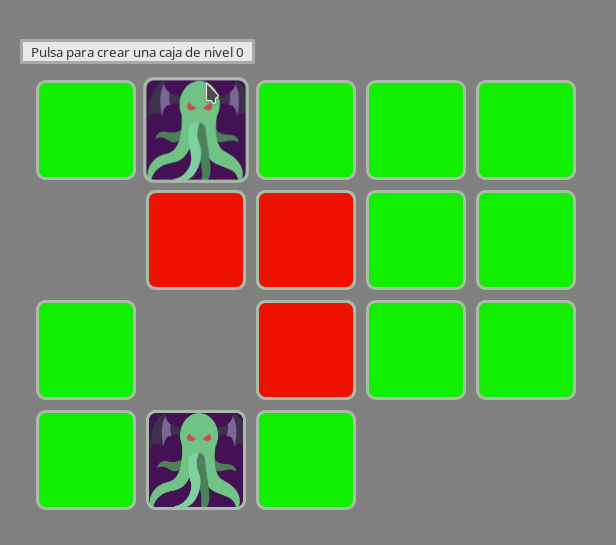
\includegraphics[width=.9\linewidth]{./imgs/Tarea_12.png}
\caption{\label{fig:restaurandoElPergamino}Ejercicio 12 - Restaurando el pergamino}
\end{figure}
\end{enumerate}
% Emacs 25.2.2 (Org mode 8.2.10)
\end{document}
